%
    \newpage
	\section[Particle-in-Cell Simulations with Monte Carlo-Collisions]%
	        {Particle-in-Cell Simulations with \\Monte-Carlo-Collisions}\label{sec:picsimulationmcc}
%
	Particle-In-Cell simulations with Monte-Carlo-Collisions (PIC-MCC) represent a powerful tool for fully kinetic plasma studies, with inclusion of complicated reaction/collision routines, as well as field solving methods. Hence they are used in all branches of plasma physics, ranging from simple labaratory discharges to electric propulsion devices and interplanetary astrophysical system. This kind of computer code simulates the motion of pseudo-particles in a continuous 1d3v-/2d3v phase-space. Macro-quantities like forces, fields and densities are stored and calculated on a mesh with constant intervals. The computational cost sums up to $N\log(N)$ per timestep --- with $N$ the total particle number --- because the self-consistent electrostatic macro-fields are calculated by solving \emph{Poisson's equation}, and no particle-particle interactions are considered.\\
	In the following section the motivation and basic scheme of a PIC-MCC simulation will be highlighted. Accordingly, the collision routines will be layed out, as well as the transition from a 1d3v to a 2d3v model. As it was mentioned in~\autoref{sec:chapter_ccrfbasics}, I will focus on the electrostatic case with $\vec{B}=0$, as the magnetic field generated from the moving charged particles is small enough that the force of $q\ix{j}(\vec{v}\ix{j}\times \vec{B})$ is negligible in comparison to $q\ix{j}\vec{E}$. 
%	
		\subsection{Principles}\label{sec:picbasics}
%
		In general, the spatio-temporal evolution of the velocity distribution function $f\ix{j}(\vec{v},\vec{r},t)$ is given by the \emph{Boltzmann equation}:
%
			\begin{align}
				\frac{\partial f\ix{j}}{\partial t}+\vec{v}\cdot\nabla_{\vec{r}}\,f\ix{j}%
					+\frac{q\ix{j}}{m\ix{j}}\vec{E}\cdot\nabla_{\vec{v}}\,f\ix{j}%
					=\left(\frac{\partial f\ix{j}}{\partial t}\right)\ix{Coll}\,.%
				\label{equ:boltzmannequation}
			\end{align}
%
			In this equation, the product of $q\ix{j}\vec{E}/m\ix{j}$ denotes the electrostatic force onto the particle of species $j$. The velocity and space gradient are calculated like $\nabla_{\vec{r}}\,f\ix{j}=\partial f\ix{j}/\partial x\cdot\vec{e}\ix{x}+\dots$ and so on. The right hand side of $(\partial f\ix{j}/\partial t)\ix{Coll}$ is the sum of all collision effects on $f\ix{j}(\vec{v},\vec{r},t)$. An approach would be an integral form, in which all probabilities of a two-body interactions with different incident and outgoing velocities are summed up in a convolution integral with $f\ix{j}(\vec{v},\vec{r},t)$.\\
			The approach via the distribution function yields the advantage of an easy access to the afore-mentioned macro-quantities, the zeroth and first moment are noted below in~\autoref{equ:zeorthandfirstmoment}. Using the moments, one can write down $f\ix{j}(\vec{v},\vec{r},t)$ at a thermodynamic equilibrium of $T\ix{j,0}$ as the \emph{Maxwell-Boltzmann-distribution-function} in~\autoref{equ:maxwellboltzmannfunction}.
%
			\begin{align}
				n\ix{j}(\vec{r},t)=q\ix{j}\int_{-\infty}^{\infty}%
					f\ix{j}(\vec{v},\vec{r},t)\diff\vec{v}\,,%
					\quad\quad%
					\langle v\ix{j}(\vec{r},t)\rangle=\frac{1}{n\ix{j}(\vec{r},t)}%
					\int_{-\infty}^{\infty}\vec{v}f\ix{j}(\vec{v},\vec{r},t)\diff\vec{v}%
				\label{equ:zeorthandfirstmoment}\\[0.3cm]
				f\ix{j}(\vec{v},\vec{r},t)=\frac{n\ix{j}(\vec{r},t)}{q\ix{j}}\,\hat{f}\ix{j}(\vec{v},\vec{r},t)%
					=\frac{n\ix{j}(\vec{r},t)}{q\ix{j}}\,{\left(\frac{m\ix{j}}{2\pi k\ix{B}T\ix{j,0}}\right)}^{3/2}%
					\,\exp\left(-\frac{|\vec{v}\ix{j}|^{2}}{v\ix{j,th}^{2}}\right)%
				\label{equ:maxwellboltzmannfunction}
			\end{align}
%
			In a Maxwellian plasma one could use a fluid dynamic approach, where the equations of motion for a single particle are multiplied with the number density function. This would reduce the computational cost drastically, as one would no longer have to track each particle individually, and sufficiently describe the discharge by charaterization of macro-quantities. This is true, if mean-free-paths are small and collisions rather likely, hence the afore-mentioned distribution function correct. In a low-temperature, low-pressure ccrf discharge mean-free-paths are large and collisions are rare, which is why a fully kinetic Particle-in-Cell simulation method is used.\\
			Satisfying the above requirements, the $n$-th equation of motion in the $N$-particle system becomes:
%
			\begin{align}
				\frac{\diff \vec{x}\ix{n}}{\diff t}=\vec{v}\ix{n}\,,%
					\quad\quad\quad%
					\frac{\diff \vec{v}\ix{n}}{\diff t}=\frac{1}{m\ix{n}}%
					\vec{F}\ix{n,L}(\vec{x}\ix{n},\vec{E},t)%
					=\frac{q\ix{n}}{m\ix{n}}\vec{E}(\vec{x}\ix{n},t)%
				\label{equ:equationofmontionpic}
			\end{align}
%
			where $F\ix{n,L}$ is the \emph{electrostatic Lorentz force}.\\
			First, the global charge density is calculted by interpolating the point charges $q\ix{n}$ of each particle onto the afore-mentioned fixed mesh grid (~\autoref{equ:interpolation}~). Next, the Poisson's equation is solved globally on that grid (~\autoref{equ:poissonpotential}~), using the interpolated density. At last, the Maxwell'is~\autoref{equ:efieldmaxwell} yields the electric field.
%
			\begin{align}
				\rho(\vec{r},t)&=\rho(\vec{x}\ix{1},\vec{x}\ix{2},\dots,\vec{x}\ix{N},t)%
					\label{equ:interpolation}\\[0.0cm]
				\Rightarrow%
				\Delta\Phi(\vec{r},t)&=-\frac{\rho(\vec{r},t)}{\varepsilon\ix{0}}%
					\label{equ:poissonpotential}\\[0.0cm]%
					\Rightarrow\hspace*{7pt}%
				\vec{E}(\vec{r},t)&=-\nabla\Phi(\vec{r},t)%
					\label{equ:efieldmaxwell}
			\end{align}
%
			The number of $N$ is of orders of magnitude higher than what the best supercomputers can handle. Hence it is assumed that one simulated particle at $\vec{x}\ix{n}$ and veloctiy $\vec{v}\ix{n}$ represents many physical particles. This \emph{superparticle factor} is usually between $\tenpo{3}$--$\tenpo{4}$, depending on the size and initial density in the simulated domain. Those superparticles follow the same dynamic and kinetic behaviour like their physical counterparts, assuming that all other relevant parameters are scaled accordingly.\\
			Furthermore, the time is also divided into discrete partitions, which yields the simulation time for a constant stept width $\Delta t$: $t\rightarrow t\ix{k}=t\ix{0}+k\, \Delta t$ (and correspondingly all other physical properties). Here, a \emph{leap frog} scheme (`Boris pusher') is used to calculate the velocities, in contrast to other time-dependent attributes, which still has a sufficient accuracy, stability and short computational time. With each calculation step, the error scales with $\sim\Delta t^{2}$ and fulfills the requirement for numerical stability $\Delta t^{\alpha>1}$. The explicit leap frog solution is calculated with old quantities of the previous timestep, thus it is simpler and faster. The single drawback on this method would be the requirement of a smaller timestep, e.g\@ $\Delta t/2$.\\
			The most significant part of the simulation code is the \emph{particle mover} or \emph{particle pusher}, in which the new positions and velocities calculated. For each particle of index $n$ and species $j$ the following equations have to be solved at a given time step $k$, or $k+/-\frac{1}{2}$ respectively:
%
			\begin{align}
				\vec{u}\ix{n,+}=\vec{v}\ix{n,k-1/2}+h\cdot\vec{E}\ix{k}\,,%
					\quad\quad%
					h=\frac{q\ix{j}}{2\,m\ix{j}}%
					\nonumber
				\end{align}\vspace*{-0.8cm}\begin{align}
				\boxed{%
					\vec{x}\ix{n,k+1}=\vec{x}\ix{n,k}+\Delta t\vec{v}\ix{n,k+1/2}%
						\quad\text{~and~}\quad%
						\vec{v}\ix{n,k-1/2}=\vec{u}\ix{n,+}+h\cdot\vec{E}\ix{k}%
						\label{equ:leapfrogscheme}%
				}
			\end{align}
%
			The field, potential and density only have to be calculated once per time step. Though this requires less effort, the calculation of $\vec{E}$, $\Phi$ and $\rho$ need to be done in this case by one processing core. The equation~\autoref{equ:interpolation} and following are solved globally. A simple approach to obtain the solution of Poisson's equation is the \emph{finite-difference method}. For a two-dimensional, with $\Delta r$ equally partitioned mesh at ($r^{(1)}\ix{l}$,$r^{(2)}\ix{m}$) one yields the \emph{five point stencil}:
%
		\begin{align}
			4\Phi\ix{l,m}-\Phi\ix{l-1,m}-\Phi\ix{l+1,m}-\Phi\ix{l,m-1}-%
				\Phi\ix{l,m+1}=\Delta r^{2}\cdot\frac{\rho\ix{l,m}}{\varepsilon\ix{0}}%
				\label{equ:fivepointstar}
		\end{align}
%
		While the potential is calculated using~\autoref{equ:fivepointstar}, all but one processing core remain idle and wait for the result to be distributed and used in the particle pusher in~\autoref{equ:leapfrogscheme}.\\
		The universal stability criteria for a kinetic plasma simulation using a PIC method with mesh size $\Delta r$ and time step $\Delta t$ are given by~\autoref{equ:stabilitycriteria}. The spatial and temporal step width should sufficiently resolve the smallest and fastest processes in the simulated model. Hence the physical scales of electron plasma frequency $\omega\ix{p,e}$ and electron Debye length $\lambda\ix{D,e}$ are chosen. The parameters are chosen so that an electron never flies beyond one cell during a single step of time. Also, the interpolation of the macro-quantities yields an error the size of micro-fluctuations between single particles, thus is negligible.
%
		\begin{align}
			\boxed{%
				\Delta t\ix{0} \le \SI{0.2}\cdot\omega\ix{p,e}%
					\quad\text{~and~}\quad%
					\Delta r\ix{0} \le \SI{0.5}\cdot\lambda\ix{D,e}%
					\label{equ:stabilitycriteria}%
				}
			\end{align}
%
			To summarize this section, a basic simulation code cycle for one time step of a PIC-MCC method is shown in~\autoref{fig:picscheme}. A more versatile and in-depth approach on PIC simulations can be found in~\cite{Tskhakaya}.
%
			\begin{figure}[!t]
				\centering
				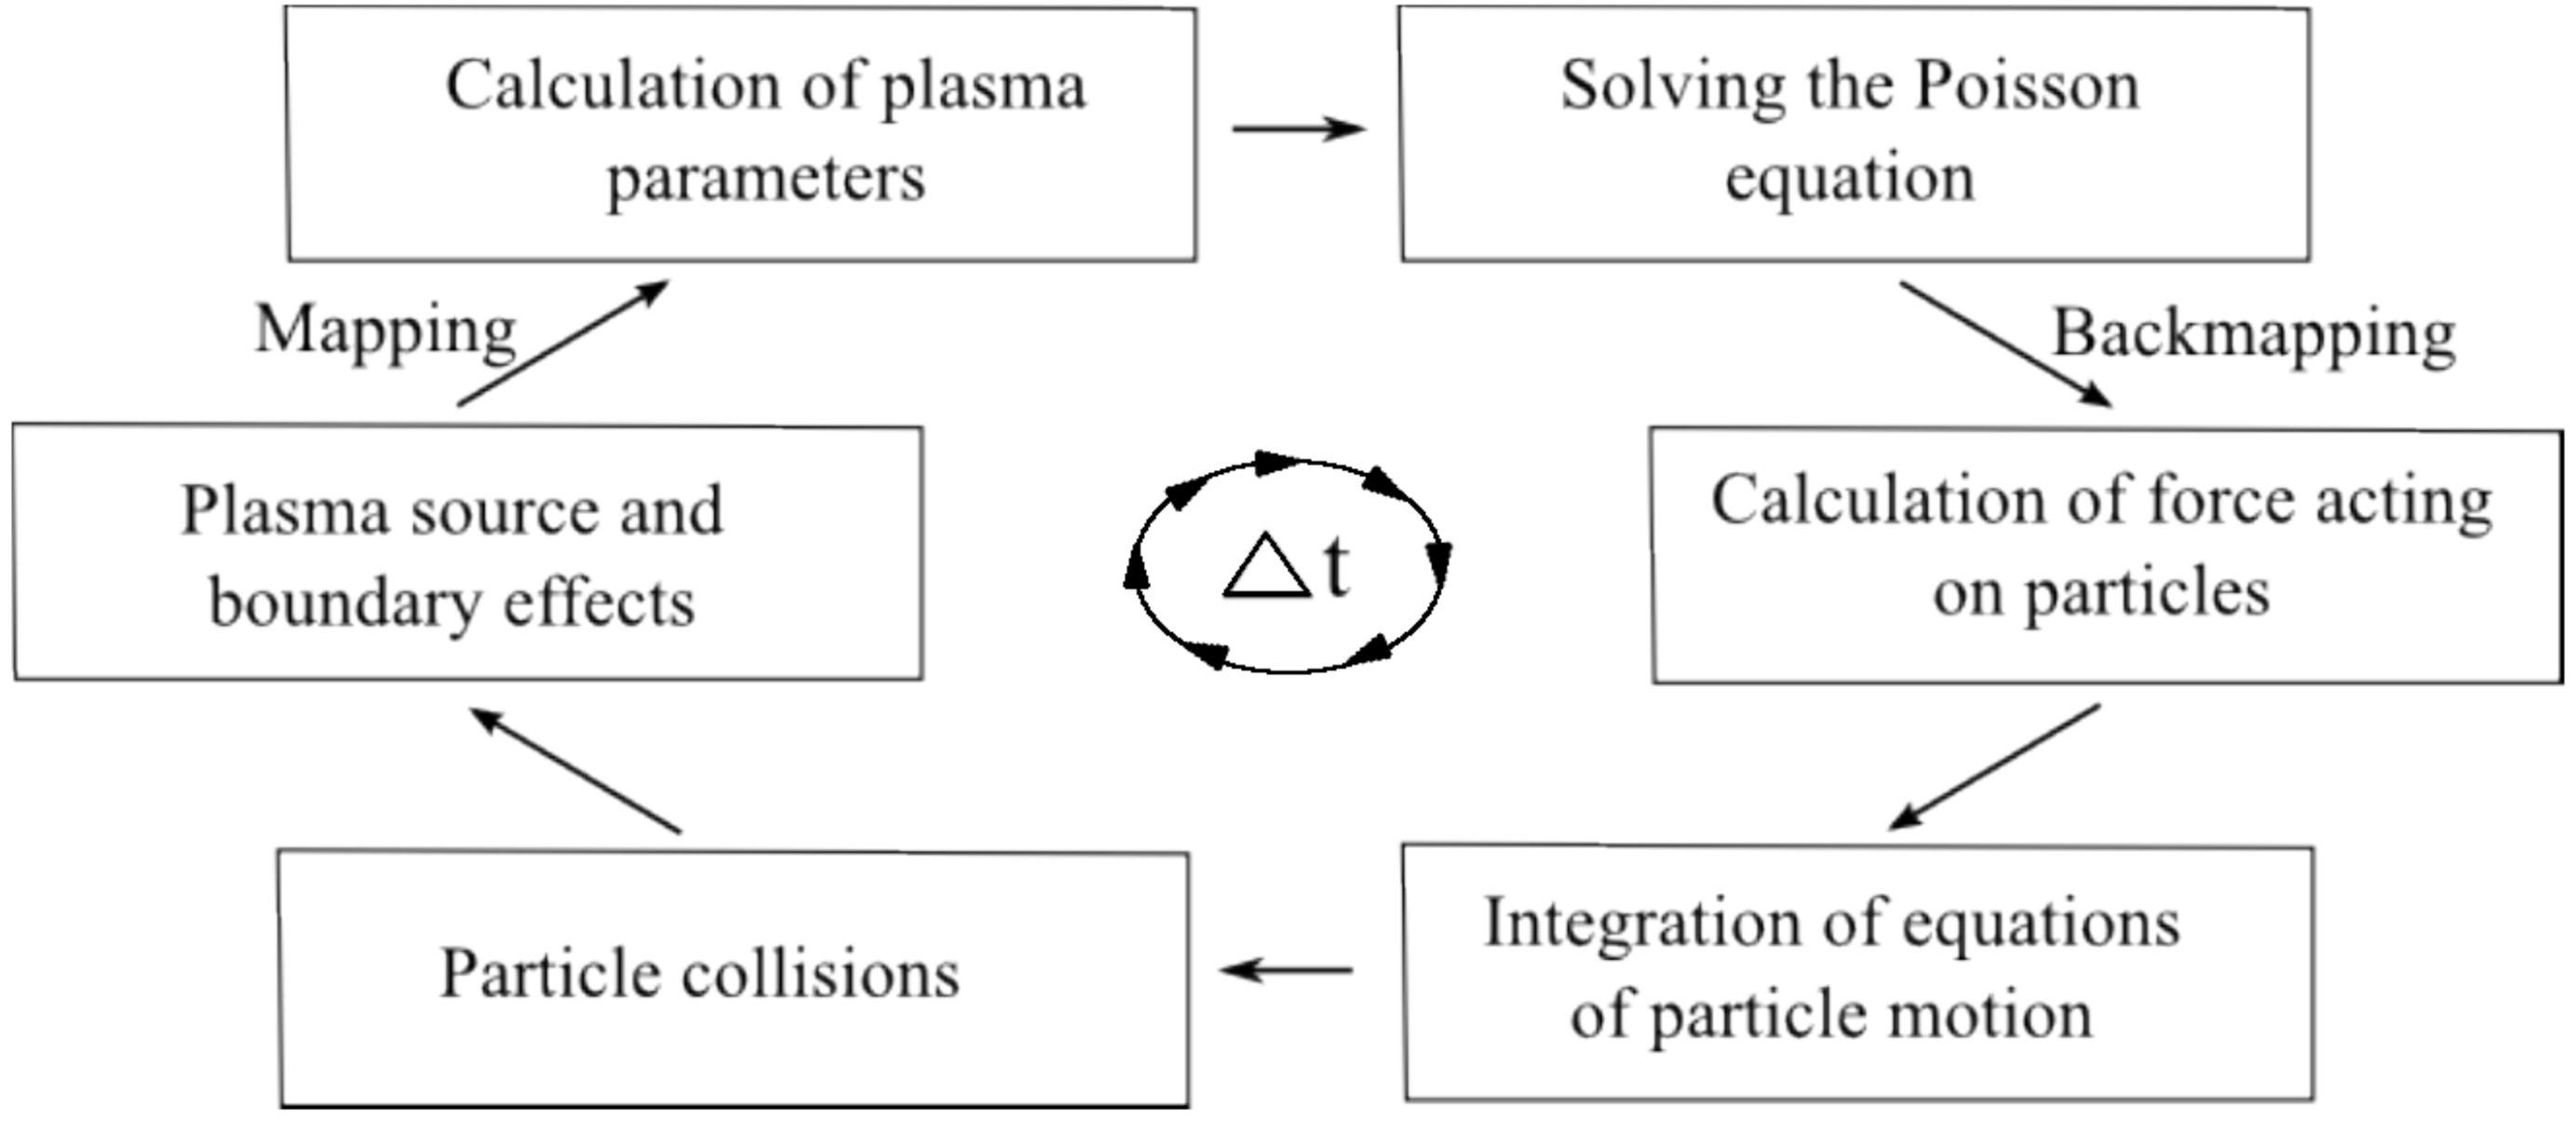
\includegraphics[width=0.8\textwidth]{figures/picscheme.pdf}
				\caption{%
				PIC simulation scheme~\cite{Matthias15}. The code starts with the initilisation of all particle species with their corresponding velocities and a first mapping process, followed by the solution of the Maxwell's equation~\autoref{equ:efieldmaxwell}. Afterwards the main loop with push, collisions, mapping and so on begins.}\label{fig:picscheme}
			\end{figure}
